

\section{Problem 4}
\label{part4}
\begin{verbatim}
Choose your (the real you, not the substitute you) favorite and
least favorite film from the data.  For each film, generate a list
of the top 5 most correlated and bottom 5 least correlated films.
Based on your knowledge of the resulting films, do you agree with
the results?  In other words, do you personally like / dislike
the resulting films?

\end{verbatim}

\subsection{Solution}
\begin{enumerate}
\item I need to choose my top favorite and least favorite movies from u.item file. For each of this film I need to find out top 5 most correlated and bottom 5 least correlated films and for that I need to give my comments.
\item I have chosen ``Die Hard (1988)'' as my top favorite film and ``Kazaam (1996)'' as my least favorite film.
\item Now I have used functions from recommendations.py to compute the top 5 correlated and least 5 correlated films.
\item I have used loadMovieLens, transformPrefs and topMatches functions from recommendations.py.
\item This in turn uses sim pearson's coefficient for getting correlation.
\item If the coefficient for each film is 1 or nearer to 1, then that film is most correlated to my film and if the coefficient is negative then that user is least correlated to my film.
\item The program for this can be found in listing\ref{lst:q4-2}.
\item Recommendations.py program can be seen in listing\ref{lst:q4-1}.
\item The output file showing sim pearson's coefficient and movie names can be seen in the fig\ref{graph41}.
\end{enumerate}
\newpage

\subsection{Code Listing}
\subsubsection{Code Listing 1}

\lstinputlisting[language=Python,breaklines = true,frame=single,caption={Python code with various functions. This is a reference code.}, label=lst:q4-1,captionpos=b,numbers=left,showspaces=false,showstringspaces=false,basicstyle=\footnotesize]{recommendations.py}
\newpage

\subsubsection{Code Listing 2}

\lstinputlisting[language=Python,breaklines = true,frame=single,caption={Python code for generating top 5 and least 5 correlated films for my top favorite and least favorite film}, label=lst:q4-2,captionpos=b,numbers=left,showspaces=false,showstringspaces=false,basicstyle=\footnotesize]{DieHard_related.py}
\newpage

\subsection{Inputs}
\subsubsection{Sample u.item file}
\begin{figure}[ht]    
    \begin{center}
        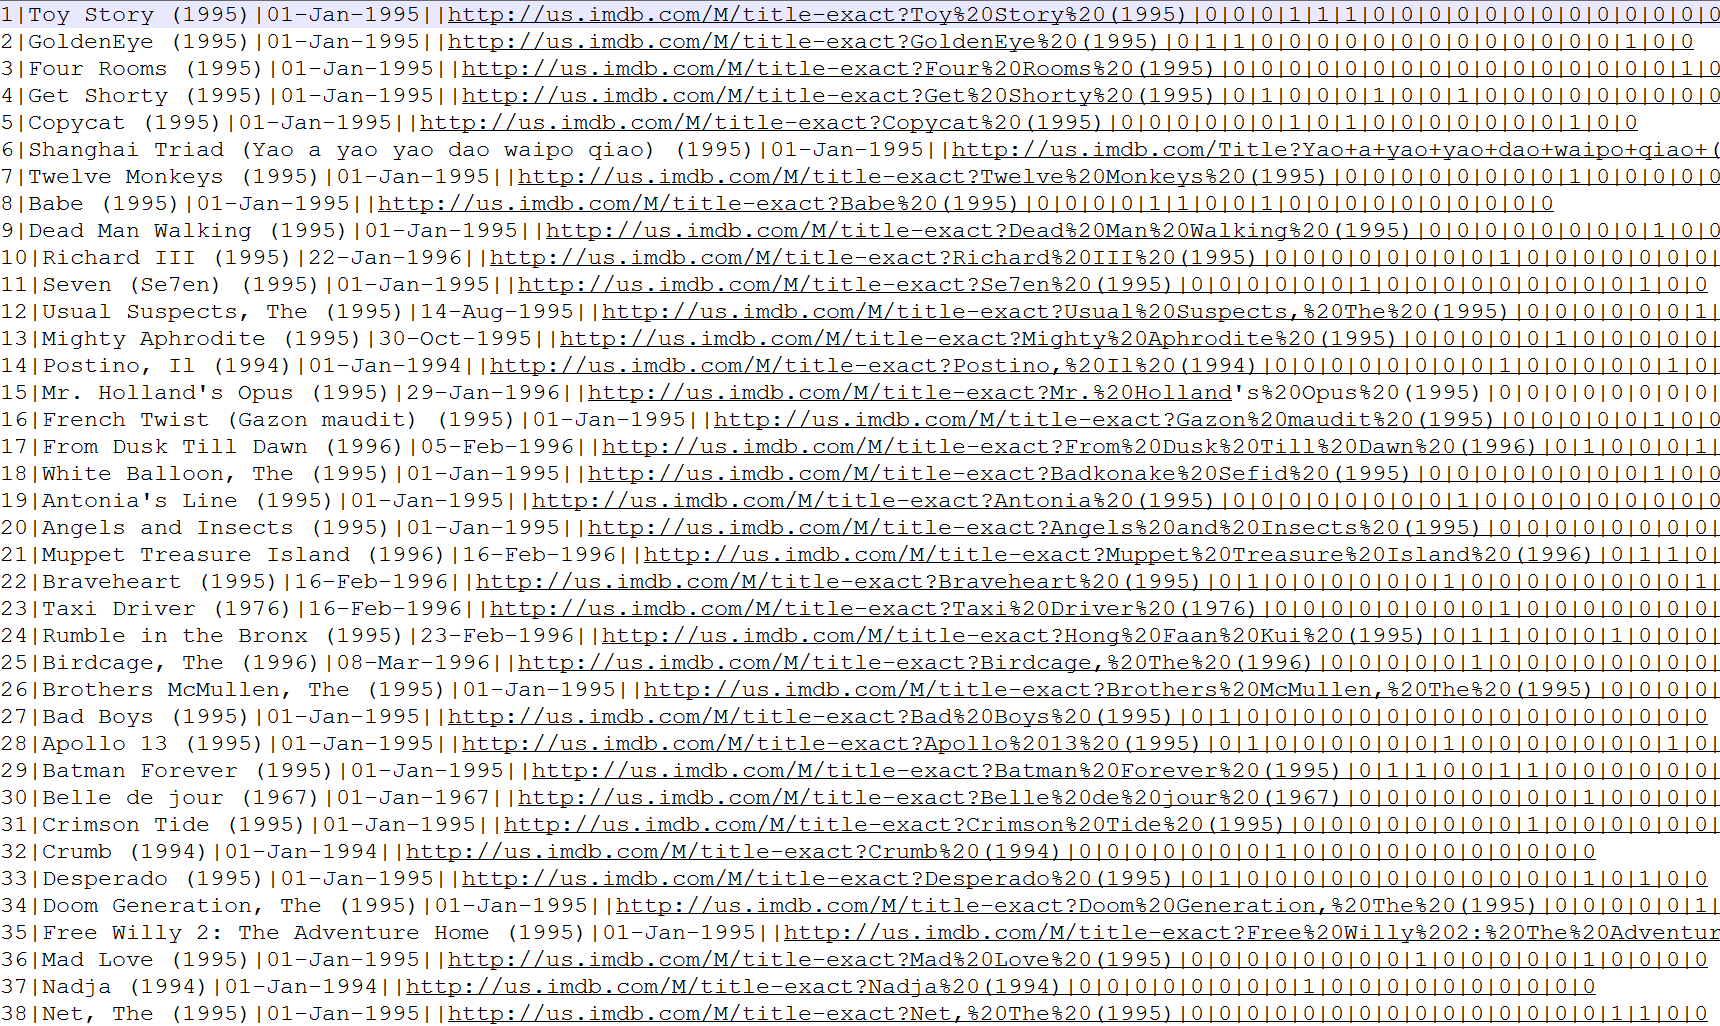
\includegraphics[scale=0.4]{sample_uitem.png}
        \caption{Sample list of movie data}
        \label{Sample4_t1}
    \end{center}
\end{figure}
\newpage
\subsubsection{Sample u.data file}
\begin{figure}[ht]    
    \begin{center}
        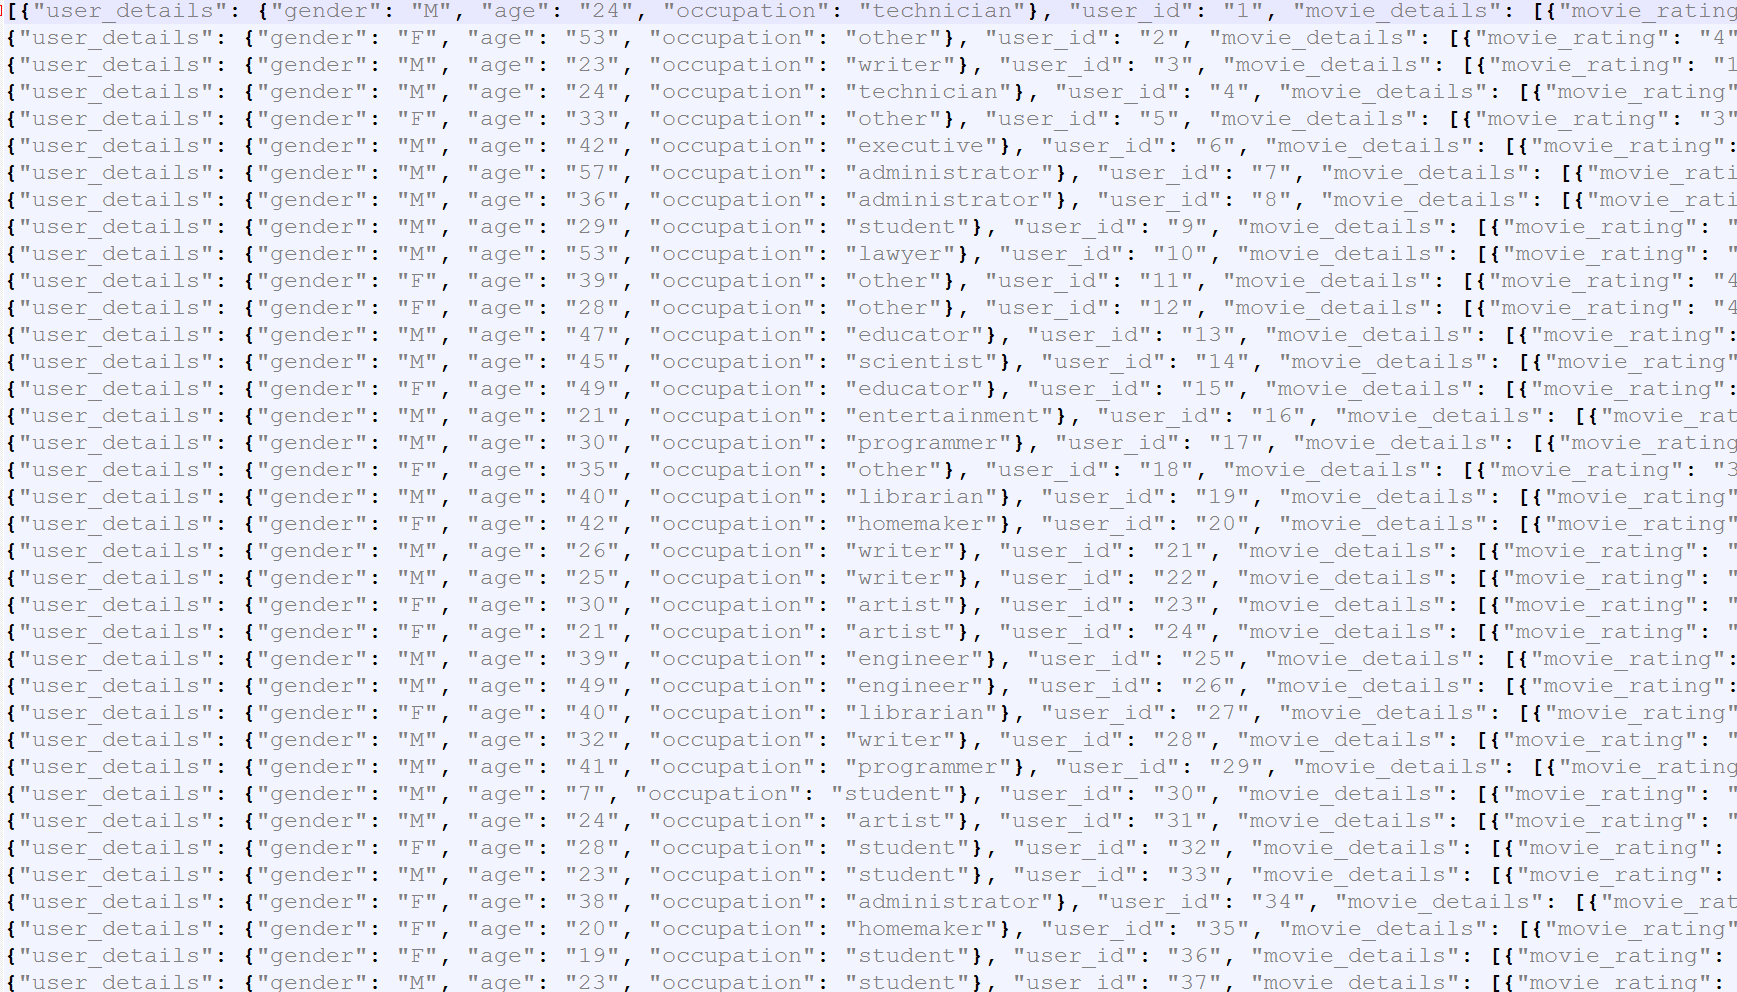
\includegraphics[scale=0.4]{sample_udata.png}
        \caption{Sample list of users and their rating for each movie}
        \label{Sample4_t2}
    \end{center}
\end{figure}
\newpage

\subsection{Output}
\subsubsection{Output file}
\begin{figure}[ht]    
    \begin{center}
        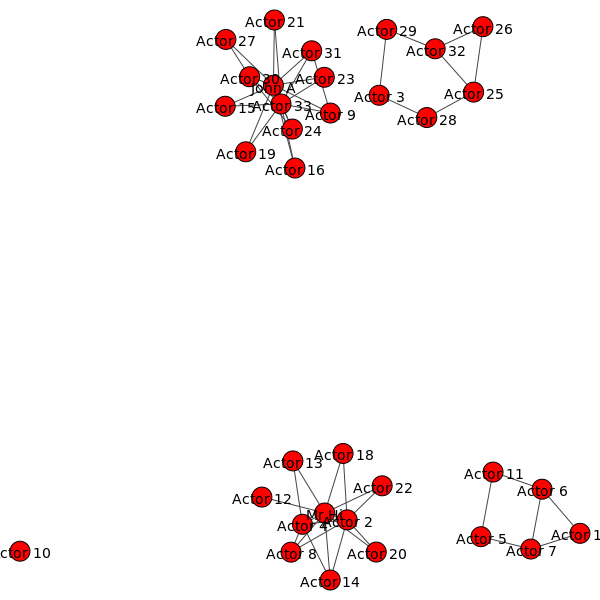
\includegraphics[scale=0.6]{output4.png}
        \caption{File contains top 5 and least 5 correlated films for my top favorite and least favorite film}
        \label{graph41}
    \end{center}
\end{figure}
\newpage
